\documentclass[11pt]{article}
\usepackage{geometry} 
\geometry{a4paper,top=3cm,bottom=3cm,left=2.5cm,right=2.5cm}   
\usepackage{multicol}
\usepackage[english, italian]{babel}
\usepackage{fancyhdr}
\usepackage{musicography}
\geometry{centering}
\usepackage{graphicx}


\pagestyle{fancy}                                 %serve ad inserire la linea sopra e il titolino
\rhead{\textsf{Lezione 3 "\textit{fondamenti dell'audio digitale 2}"}}
\renewcommand{\headrulewidth}{5pt} %grandezza della linea in alto
\renewcommand{\footrulewidth}{1pt}   % grandezza della linea in basso


\begin{document}
\begin{minipage}{0.55\linewidth}
\vspace{0.3cm}
{\large{\textbf{\textsf{Gabriele Petrillo}}}}\\\end{minipage}

\vspace{0.3cm}
\begin{minipage}{0.95\linewidth}
\begin{center}
{\huge{\textbf{\textsf{Fondamenti dell'audio digitale 2}}}} \\
\end{center}
\end{minipage}
\vspace*{0.2cm}


%=========ABSTRACT=======================
\begin{center}
\begin{minipage}[c]{14cm}
\begin{textit}

Ciò che segue è stato sviluppato a partire dalla dispensa di composizione del 09/12/2019 del prof. N.Bernardini presso il conservatorio S.Cecilia di Roma che possono essere consultati presso https://github.com/SMERM/TR-2019-2020/tree/master/A.A.2019-2020/COME-02/20191209. L'argomento trattato sono i Decibel e la quantizzazione di un segnale audio con dimostrazioni ed esempi in Octave.

\end{textit}
\end{minipage}
\end{center}
\vspace*{0.2cm}

%=========ARTICOLO========================

\begin{multicols*}{2}
\parskip=0pt

\textbf{\textsf {Decibel}}\\

\noindent Il Decibel è un'unità di misura logaritmica del rapporto tra due grandezze omogenee. Viene generalmente usato per misurare i fenomeni acustici ed esprime varie unità di misura, il pascal, il volt, il watt, a seconda del tipo di dB preso in considerazione. La caratteristica del decibel è quella di rappresentare i dati in modalità logaritmica e questo permette di descrivere grandi variazioni numeriche, come la pressione sonora, con numeri  di poche cifre. L'espressione matematica è:
\[
dB = 10 * log_{10}(liv./liv. \, di \, riferimento)
\]

Il dBSPL (sound pressure level) è una scala usata per misurare il livello di pressione sonora. È la grandezza utilizzata per esprimere il livello di pressione del suono rispetto la soglia di udibilità. La scala parte da 0 dB, che rappresenta la soglia di udibilità, ed arriva a circa 125 dB che rappresenta la soglia del dolore - ovvero la massima pressione sonora udibile in modo continuato senza creare danni all'apparato uditivo\footnote{In realtà la scala arriva a circa 194 dB che rappresenta il limite fisico, ma rappresentano livelli di pressione sonora che non sono utili alla nostra trattazione.}.

Bisogna tener presente che essendo una grandezza logaritmica ogni raddoppio della pressione acustica è rappresentata da soli 6dB - quindi il doppio di 4o dBSPL sarà 46 dBSPL.\\

\textbf{\textsf {Il Range Dinamico}}\\

\noindent il range dinamico è espresso in decibel e rappresenta la differenza tra il livello più alto e quello più basso di un segnale. Nel caso di un sistema digitale rappresenta il più alto livello sonoro rappresentabile senza distorsioni e il rumore di fondo dei componenti elettronici. 

Una grandezza associata al range dinamico è il rapporto segnale/rumore (SNR), ovvero il rapporto tra il segnale più forte possibile ed il rumore di fondo. Più il rapporto è ampio e più il suono risulterà chiaro. In condizioni ottimali il range dinamico è uguale al SNR.\\

\textbf{\textsf {Quantizzazione}}\\

\noindent Un altro passaggio del processo di conversione è la quantizzazione, ovvero l'accuratezza con cui è misurato il valore numerico di ogni campione. I valori di un segnale campionato possono assumere solo valori che possono essere rappresentati dalla memoria del computer, in genere numeri interi. I valori dei campioni vengono quindi arrotondati per difetto al valore più vicino rappresentabile. Per esempio, supponendo che il convertitore D/A è capace di rappresentare un segnale ad intervalli di  0.001V. Se un campione è campionato a 0.01227 V, sarà convertito a 0.012 V - con un errore di 0.00027 V. \\

\textbf{\textsf {Rumore di quantizzazione}}\\

\noindent Il valore di ogni campione differisce leggermente dal valore del segnale originale e questo problema è conosciuto come errore o rumore di quantizzazione. La quantità e l’effetto udibile dell’errore dipende dalla risoluzione del convertitore e dal tipo di segnale in ingresso. Per esempio, se un convertitore A/D lavora con 12 bit si avrà in uscita di $2^{12} = 4096$ possibili valori. Supponendo che il segnale audio in ingresso può variare tra -10 e +10V - per un range totale di 20V, la grandezza dell'intervallo di quantizzazione corrispondente al valore di un bit sarà $20/4096 = 0.004883$ V/bit.
 Questo errore si mostra generalmente come un fruscio (white noise), tuttavia può manifestarsi in maniera diversa a seconda del tipo di segnale in ingresso al convertitore.
 
 Se il segnale è molto basso di livello si possono verificare dei troncamenti che creano delle armoniche non presenti nel segnale originali che potrebbero superare la frequenza di Nyquist e creare delle frequenze di alias.

Per eliminare il problema è possibile inserire del rumore bianco a bassissimo livello (la quantità di rumore aggiunto in genere è dell'ordine di 3 dB) in modo da mascherare le frequenze spurie che si vengono a creare in seguito al troncamento del sengnale, questo rumore è chiamato \textit{dither}. È possibile anche aumentare la risoluzione dei bit per avere un range dinamico più grande e far ricadere gli artefatti ad un livello non udibile. Aumentando la risoluzione in bit almeno a 20 avremo infatti almeno 120 dB di dinamica in modo da eccedere il range dinamico percepibile dall'uomo in qualsiasi ambiente.\\

\textbf{\textsf {Il range dinamico in un sistema digitale}}\\

Per calcolare il massimo range dinamico di un sistema digitale, possiamo usare la seguente formula:
\[
Max.\, range\, dinamico\, in\, dB = n. bit * 6
\]

Il numero 6 deriva dal fatto che ogni bit di risoluzione rappresenta 6 dB di dinamica. Quindi, se registriamo un suono con un sistema ad 8 bit avremo un range dinamico di 48 dB, se registriamo a 16 bit, il range dinamico aumenta a 96 dB. Un convertitore a 20 bit offre un range dinamico di 120 dB, che corrispondo all’incirca a quello dell’uomo.\\

\textbf{\textsf {Ex.1 Simulazione di segnale quantizzato a 2 3 4 8 12 16 bit}}\\

\begin{center}
\begin{minipage}[c]{6.3cm}
\begin{sffamily}

[snd fc] = audioread ("babay.wav");\\
nbits = [2 3 4 8 12 16];\\
out = zeros (length(snd) * \\
lenght(nbits),1);\\
dur = length(snd)/fc;\\

for k = 1:length(nbits)\\
curbits = 2\textasciicircum nbits(k);\\
curstep = 2/curbits;\\
globstart = (length(snd)*(k-1)) + 1;\\
tmpout = round(snd / curstep)*\\
curstep;\\
out(globstart : globstart + \\
length(tmpout)-1) = tmpout;\\
end\\
audiowrite("babaynew.wav",out,fc)\\

\end{sffamily}
\end{minipage}
\end{center}

\noindent Cerchiamo di leggere il codice velocemente senza soffermarci sul funzionamento degli opcode già descritti nella lezione precedente. 

Per prima cosa dobbiamo leggere il file audio da ricampionare attraverso la funzione \textit {audioread}. Scriviamo un array \textit {nbits} con la profondità di bit che vogliamo utilizzare ad ogni ciclo. Costruiamo una matrice \textit {out} grande quanto \textit {snd} * il numero di elementi di \textit {nbits} - il prodotto tra il file campionato ed il numero di volte che verrà riquantizzato  - che sarà la matrice di output con conterrà i nuovi campioni. Ed infine stabiliamo la durata in secondi del file con la variabile \textit{dur}.

Ora dobbiamo creare il ciclo che leggerà il file con i diversi valori di quantizzazione. Possiamo leggerlo così per K uguale a 1 arriva al numero di elementi presente in \textit {nbits} - che rappresenta il numero di volte che dobbiamo rileggere il file.

Ora dobbiamo specificare per ogni ciclo - quindi per ogni valore di k - la quantità di valori di quantizzazione secondo la formula $2^{nbits}$ il valore di ogni step $2/quantità\, step& quindi:

\begin{center}
\begin{minipage}[c]{6.3cm}
\begin{sffamily}

curbits = 2\textasciicircum nbits(k);\\
curstep = 2/curbits;\\

\end{sffamily}
\end{minipage}
\end{center}

Con k stabiliamo la posizione dell'elemento nell'array \textit {nbits}.

Con \textit {globalstart}\footnote{Per la spiegazione di globalstart guardare lez_1 Ex_4} identifichiamo il campione di inizio di ogni ciclo.

Ora dobbiamo riquantizzare tutti i campioni, la formula è:
\[
x_{qnt} = [x/q]*q
\]

dove $x_{qnt}$ è il segnale quantizzato, x sono i campioni originali - nel nostro caso \textit {snd} e \textit q è il valore degli step di campionamento, quindi \textit{curstep}.

quindi:

\begin{center}
\begin{minipage}[c]{6.8cm}
\begin{sffamily}

tmpout = round(snd/curstep)*curstep;\\

\end{sffamily}
\end{minipage}
\end{center}

Per finire dobbiamo scrivere i valori nella nostra matrice di uscit \textit {out} copiando i valori ti tmpout nelle posizioni che vanno da \textiti {globalstart} - il campione di inizio - alla lunghezza di \textit{tmpout} - tutta la lunghezza dei nuovi campioni, successivamente \textit {audiowrite} scriverà il nuovo file audio:

\begin{center}
\begin{minipage}[c]{6.8cm}
\begin{sffamily}

out(globstart : globstart + \\
length(tmpout)-1) = tmpout;\\
end\\
audiowrite("babaynew.wav",out,fc)\\

\end{sffamily}
\end{minipage}
\end{center}

Lo script produce il seguente plot:

\begin{center}
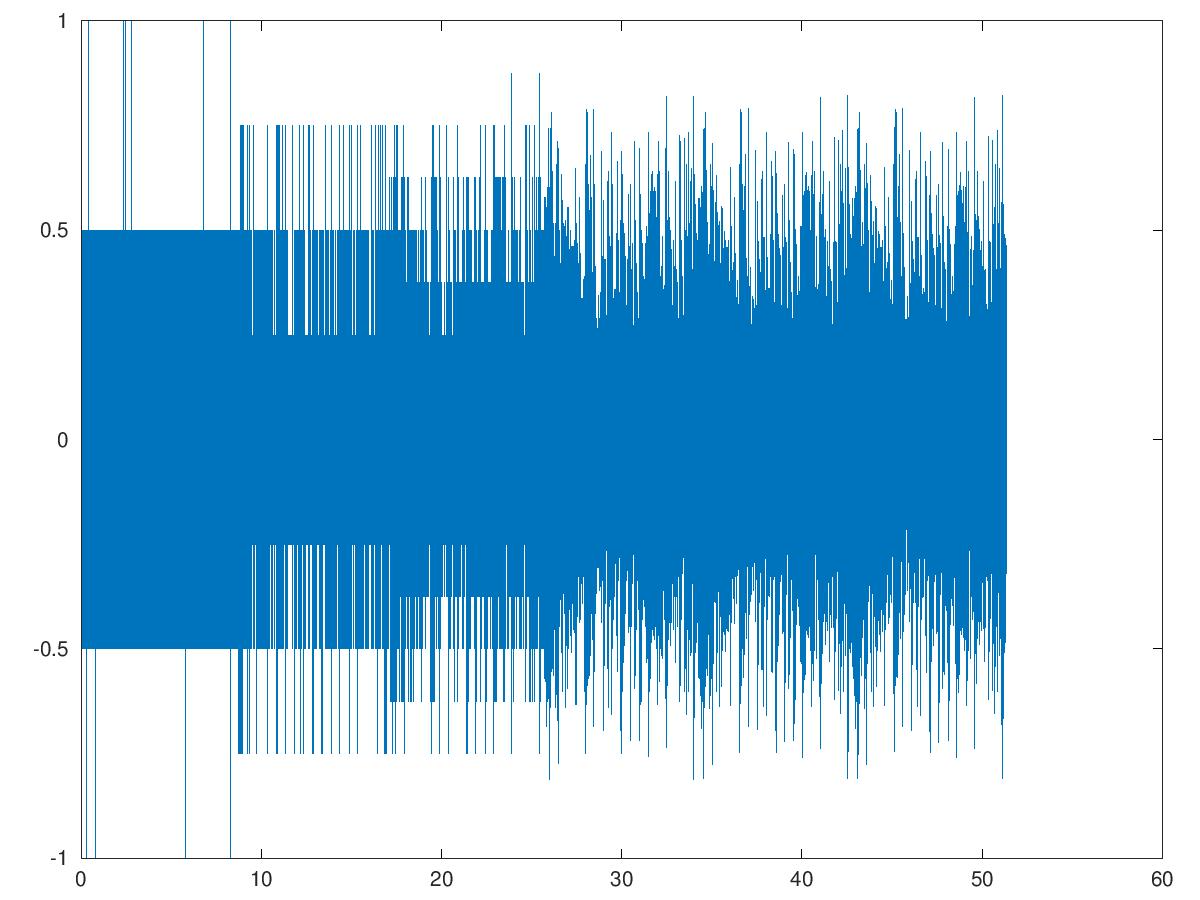
\includegraphics[scale=0.4]{images/plot01.png}

{\scriptsize \emph{fig.1 }}
\end{center}

\vspace{3cm}

\textbf{\textsf {Ex.2 Calcolo dell'errore di quantizzazione}}\\

\noindent Cerchiamo di calcolare l'errore di quantizzazione di un segnale. Per calcolare l'errore di quantizzazione dobbiamo applicare la formula:
\[
z_{errore} = x_{sig} - x_{qnt}
\]

dove \textit z - l'errore di quantizzazione - è uguale alla differenza tra segnale in ingresso \textit {$x_{sig}$} e il segnale quantizzato \textit {$x_{qnt}$}.

\begin{center}
\begin{minipage}[c]{6.3cm}
\begin{sffamily}

[snd fc] = audioread ("babay.wav");\\
nbits = [2 3 4 8 12 16];\\
out = zeros (length(snd) * \\
lenght(nbits),1);\\
dur = length(snd)/fc;\\

for k = 1:length(nbits)\\
curbits = 2\textasciicircum nbits(k);\\
curstep = 2/curbits;\\
globstart = (length(snd)*(k-1)) + 1;\\
tmpout = round(snd / curstep)*\\
curstep;\\
dif = snd - tmpout;\\
out(globstart : globstart + \\
length(tmpout)-1) = dif;\\
end\\
audiowrite("babaydif.wav",out,fc)\\

\end{sffamily}
\end{minipage}
\end{center}

Questo codice è uguale al precedente in cui però è stato implementato il calcolo dell'errore di quantizzazione e la matrice di output è stata uguagliata all'errore, così possiamo stampare l'errore:

\begin{center}
\begin{minipage}[c]{6.3cm}
\begin{sffamily}

dif = snd - tmpout;
out(globstart : globstart + \\
length(tmpout)-1) = dif;\\

\end{sffamily}
\end{minipage}
\end{center}

lo script produce il seguente plot:

\begin{center}
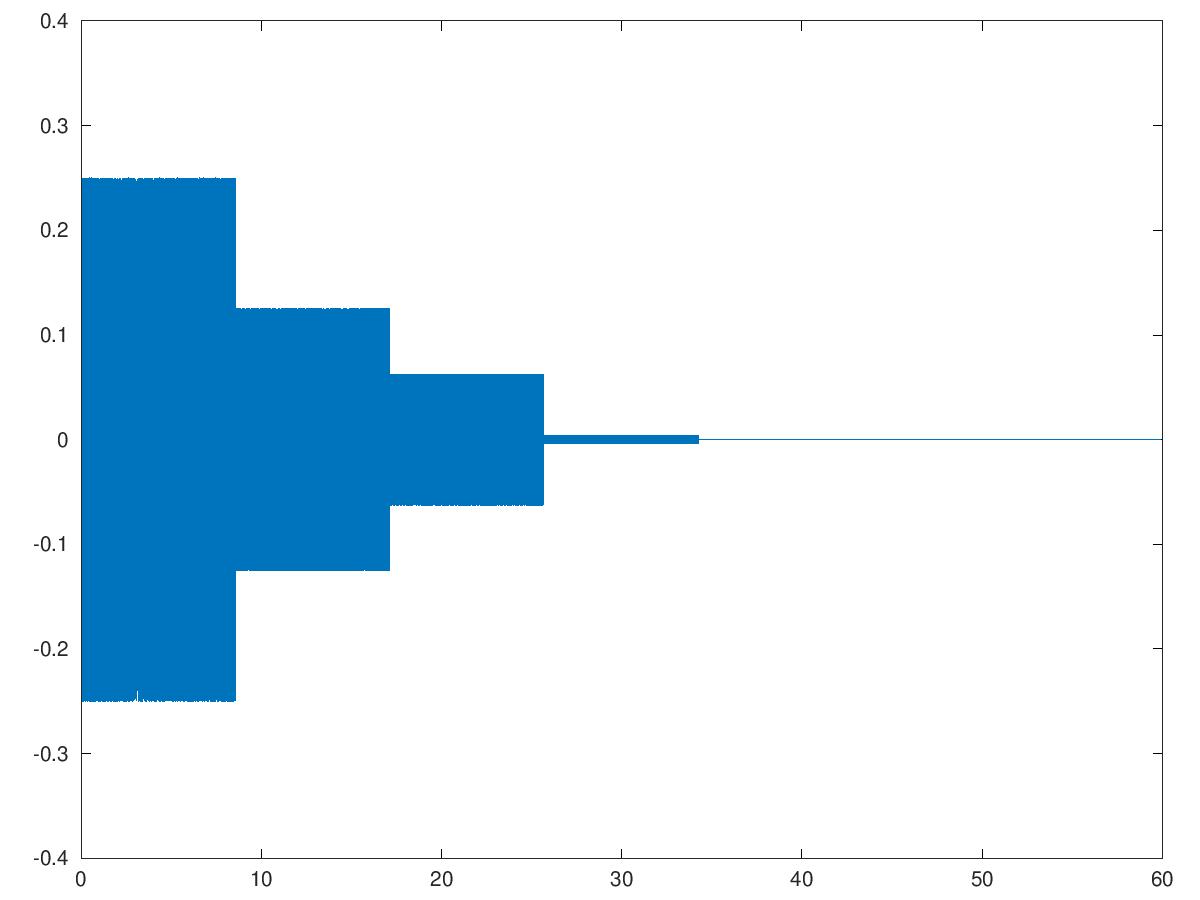
\includegraphics[scale=0.4]{images/plot02.png}

{\scriptsize \emph{fig.2 }}
\end{center}

Da questo plot possiamo vedere che alla fine non abbiamo nessun errore di quantizzazione, questo avviene perchè il file di origine non è un segnale analogico, ma digitali campionato a 16 bit.

\section*{\centering\small{BIBLIOGRAFIA}}
•\textsc{\textsf {Dodge, Charles and Jerse, Thomas A}}, \emph{Computer music: synthesis, composition and performance}, Macmillan Library Reference 1997\\
•\textsc{\textsf {Roads, Curtis and Strawn, John and others}}, \emph{The computer music tutorial}, MIT press, Editor 1996\\
•\textsc{\textsf {Massimi, Marco}}, \emph{Mastering in the box}, Contemponet 2018\\

\end{multicols*}

\end{document}